[48 v\textsuperscript{o}] Quod tamen ope magnetis\protect\index{Sachverzeichnis}{magnes} etiamsi summe corrigatur, etiamsi inveniatur ratio medendi declinationibus, haberi \textso{non} potest. Imo etsi inventae essent longitudines\protect\index{Sachverzeichnis}{longitudo} et latitudines\protect\index{Sachverzeichnis}{latitudo} tum naves\protect\index{Sachverzeichnis}{navis} non possent incedere lineis rectis, sed tenerentur moveri curvis. Sed nunc ea ratione perfectum est demum histiodromice. Nec potest magis perfici, nisi quis instrumentum inveniat idem subtilius per aerem efficiendi, atque nos per aquam, id enim esset commodius.\pend \pstart Hoc quoque probe observandum, ut pendeant omnia horologia\protect\index{Sachverzeichnis}{horologium} et machinae, ut quantumcunque jactetur navis, maneant tum semper in situ horizonti parallelo. Quod ideo fieri non difficulter potest, quia alioqui omnia a nave\protect\index{Sachverzeichnis}{navis} libera sunt, et in aliam quam ipsa parte vertuntur, eodem modo et nauticae pyxidis\protect\index{Sachverzeichnis}{pyxis!nautica} capsula pondere plumbeo supposito semper constituitur horizonti parallela.\pend \pstart Aqua sane commoda est ad cursum, sed non ad flexum navis\protect\index{Sachverzeichnis}{navis} ostendendum. Quia ita includi non potest, sed libera simul et stabilis esse debet. Quod ob maris continuos motus obtineri non potest. Ergo alia media cogitavi quibus aliquid in navi sit, quod circumgyrante sese nave, non circumgyretur. Sed initio Magnetem\protect\index{Sachverzeichnis}{magnes} elegeram, qui sufficeret sane, nisi plus aliquid molirer, non solum inventionem Longitudinum\protect\index{Sachverzeichnis}{longitudo}, sed et \pgrk{>'orjwsin t~hs loxodrom'ias}. Ergo sic animum induxi. Venit ergo in mentem saepe contingere \edtext{ut}{\lemma{contingere}\Afootnote{ \textit{ (1) }\ non solum \textit{ (2) }\ ut \textit{ L}}} aliquid ab alio pendeat, et tamen eo circumacto non circumagatur, sed renitatur ob gravitationem\protect\index{Sachverzeichnis}{gravitas}. Et cogitavi id optime fieri, si suspendens et suspensum se tangant in paucis punctis, vel fere in uno ut in duabus sphaeris sibi impositis. Si ambae sint circa eundem axem, et inferior sit parva et in illo axe firmata, superior sit magna et libera, posse superiorem cum axe circummoveri, immota superiore. Ita h.l. fiet axis duarum sphaerarum.\label{fig3}
   \begin{wrapfigure}{l}{0.65\textwidth}
   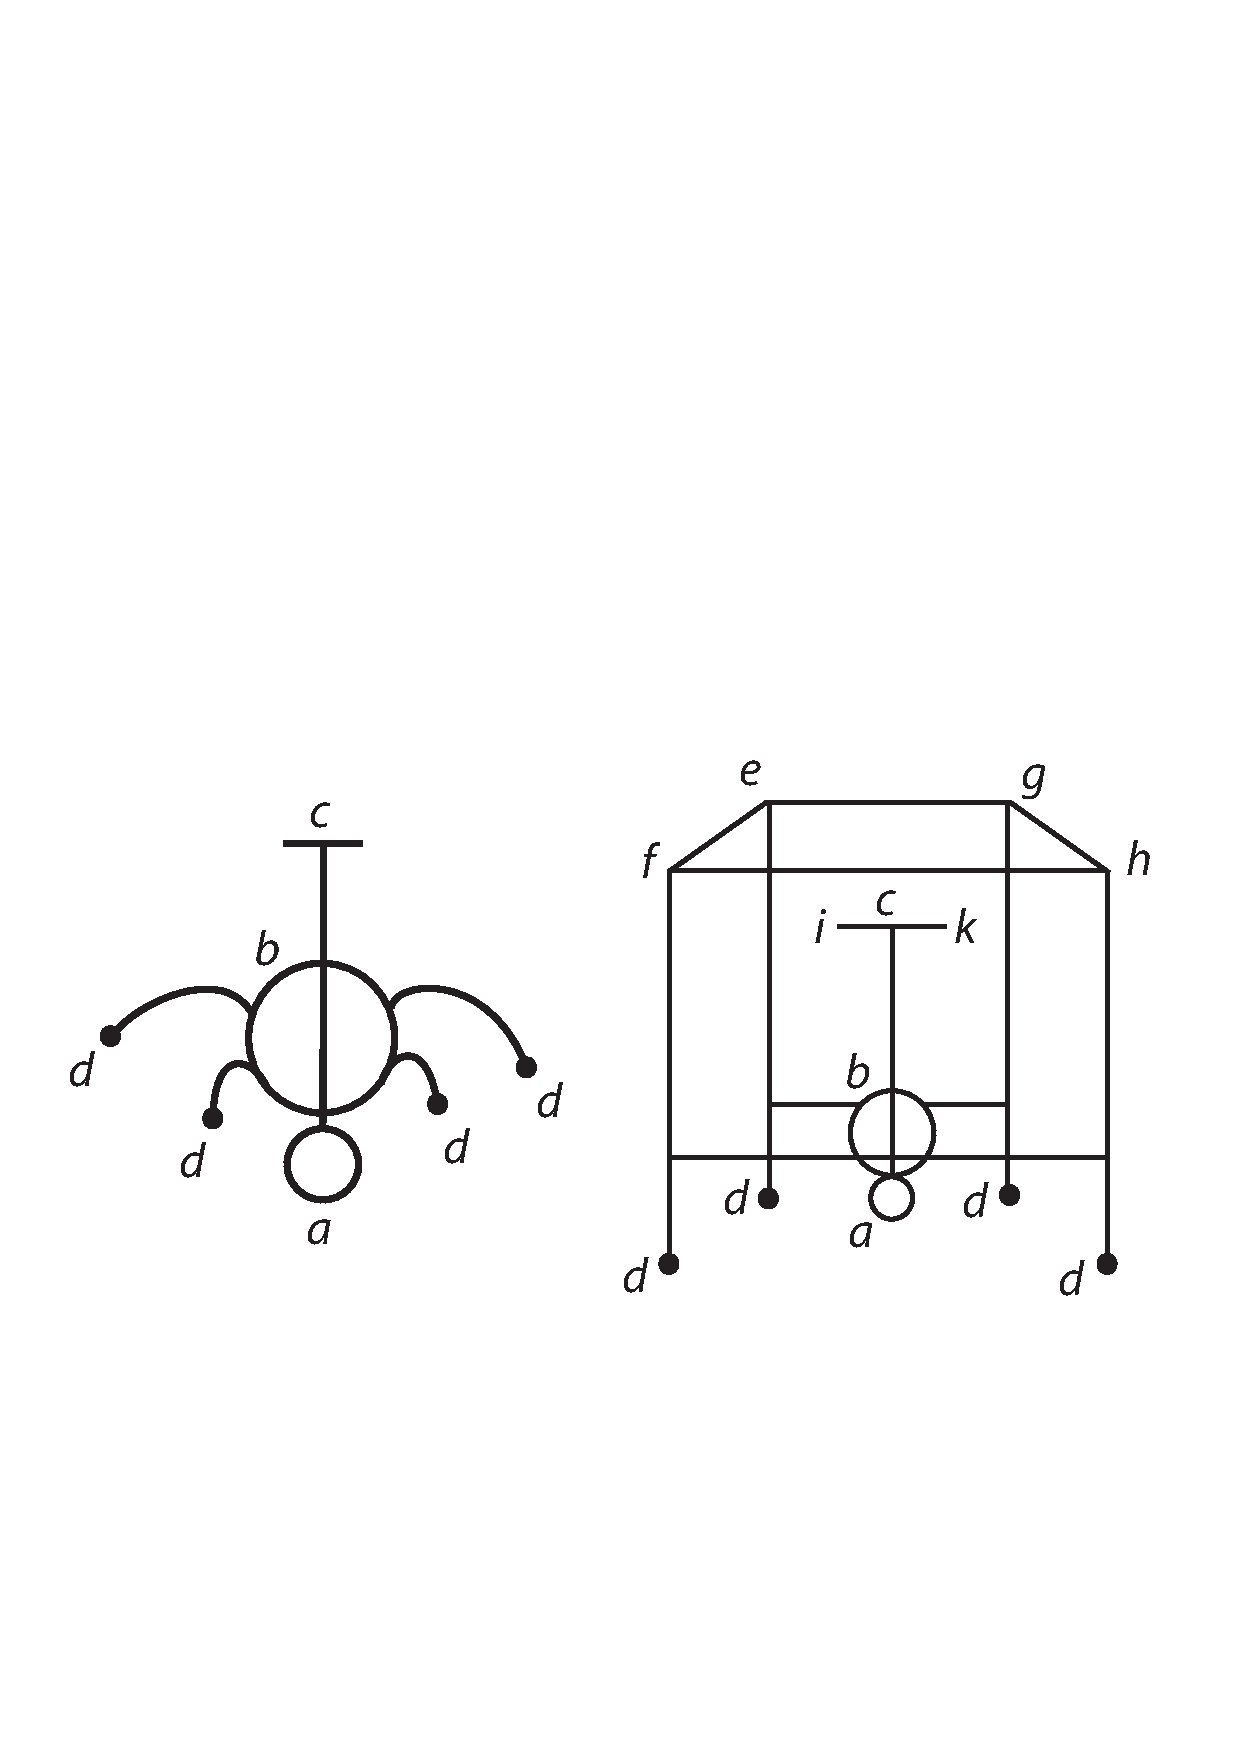
\includegraphics[width=0.65\textwidth]{images/35_15_6_48v1u2}\\
   \hspace{10mm} \textit{[Fig. 2, gestrichen]}\hspace{30mm}\textit{[Fig. 3]}
   \end{wrapfigure}
Sit communis cum axi \edtext{navis\protect\index{Sachverzeichnis}{navis} mentali}{\lemma{navis}\Afootnote{ \textit{ (1) }\ et axis sp \textit{ (2) }\ mentali \textit{ L}}}. Axis duarum sphaerarum ita sit ut \edtext{superius liber}{\lemma{}\Afootnote{superius liber \textit{ erg.} \textit{ L}}} possit se collocare perpendiculariter ad horizontem, sphaerae sint ex materia laevi, v.g. politissmo aere aut marmore. Sphaeras transeat ille axis. Inferior sphaera sit \textit{a} superior \textit{b}. Locus a quo axis \textit{ac} pendet sit \textit{c}. Axis sit linea rigida firmus cum \textit{a} sphaera. Sed \textit{b} sphaeram transeat non tamen tangat. Ex sphaera \textit{b} pendeant \edtext{lineis rigidis}{\lemma{}\Afootnote{lineis rigidis \textit{ erg.} \textit{ L}}} plurima pondera \textit{d} ut tanto sit gravior ita tamen ut sustineri possit per axem. Eo\edtext{}{\lemma{}\Afootnote{Eo \textbar\ tamen \textit{ gestr.}\ \textbar\ cum \textit{ L}}} cum motu navis\protect\index{Sachverzeichnis}{navis} se circumagente movebitur cum eo sphaera inferior \textit{a} immota superiore \textit{b} ejusque ponderibus. Ex singulis 4 ponderibus sphaerae \textit{b} prodeant lineae rigidae \textit{de}, \textit{df}, \textit{dg}, \textit{dh} portantes tabulam \textit{efgh}, quae proinde circumacta nave\protect\index{Sachverzeichnis}{navis} \edtext{non}{\lemma{nave}\Afootnote{ \textit{ (1) }\ et sp \textit{ (2) }\ non \textit{ L}}} circumagetur sed perpetuo retinebit eundem situm ad \edtext{locum relictum et quaesitum}{\lemma{locum}\Afootnote{ \textit{ (1) }\ discessus et abscessus \textit{ (2) }\ relictum et quaesitum \textit{ L}}}.\footnote{\textit{In der rechten Spalte}: NB. Forte effici et constantia plagae posset, si arte magnetica exhiberi posset res in aere pendens sine fulcro in vitro hermetice clauso, ne aer corrumpat vim contrariorum magnetum\protect\index{Sachverzeichnis}{magnes} ita tamen ut propelleret rem non tamen verteret. Forte idem praestabile illa quasi pendulatione qua Kircherus 
 %\edtext{}{\lemma{Kircherus}\Bfootnote{\textsc{A. Kircher}, \textit{Magnes}, Rom 1554, S. 309.}}
\protect\index{Namensregister}{\textso{Kircher} (Kircherus), Athanasius SJ 1602\textendash 1680} rem subtilissimo filo alligatam a magnete\protect\index{Sachverzeichnis}{magnes} facit sursum latam, quae ita etiam quasi pendulum\protect\index{Sachverzeichnis}{pendulum} apparet, nam sane circumacto licet fili fulcro, etiam contracto paulum filo ferrum tamen ipsum manet \protect\index{Sachverzeichnis}{magnes} intactum, si hujus rei stabilitas effici potest, iterum vicinius. }\pend \pstart Hac ratione suppletur defectus Magnetis\protect\index{Sachverzeichnis}{magnes}. Magnes\protect\index{Sachverzeichnis}{magnes} enim retinet semper (declinationibus\protect\index{Sachverzeichnis}{declinatio} demtis) eundem situm ad plagas mundi, sed hoc instrumentum retinet semper eundem situm ad locum relictum et quaesitum, et ita ea ratione retento eodem versorii nostri situ licebit linea recta currere, cum contra qui magnetis\protect\index{Sachverzeichnis}{magnes} versorium sequitur, si quidem linea recta currere vult mutabit quovis prope momento situm magnetis\protect\index{Sachverzeichnis}{magnes}; sin vult magnetis \protect\index{Sachverzeichnis}{magnes} situm retinere, \edtext{nunquam}{\lemma{retinere,}\Afootnote{ \textit{ (1) }\ et ita \textit{ (2) }\ regulam \textit{ (3) }\ nunquam \textit{ L}}} movebitur linea recta ad locum destinatum. Muniri debet hoc in$\langle$str$\rangle$umentum ab omni extraneo impulsu et aere.  Hoc instrumento efficietur ut sine coelo, stellis\protect\index{Sachverzeichnis}{stella} et magnete\protect\index{Sachverzeichnis}{magnes} determinari possit locus navis\protect\index{Sachverzeichnis}{navis}, longitudo \protect\index{Sachverzeichnis}{longitudo} et latitudo\protect\index{Sachverzeichnis}{latitudo}, distantia, cursus, celeritas\protect\index{Sachverzeichnis}{celeritas}, \edtext{}{\lemma{}\Afootnote{celeritas, \textbar\ etsi nullus adsit compassus, \textit{ gestr.}\ \textbar\ flexus, \textit{ L}}}flexus, tempus, et quid non? Cognita tantum longitudine\protect\index{Sachverzeichnis}{longitudo} et latitudine\protect\index{Sachverzeichnis}{latitudo} loci discessus et quaesiti \pend \pstart Hoc olim potuissent veteres supplere defectum magnetis\protect\index{Sachverzeichnis}{magnes}. Constat enim nulla peculiari naturae observatione, sed meris principiis \edtext{mechanicis}{\linenum{|20|||20|}\lemma{Kircherus}\Bfootnote{\textsc{A. Kircher}, \textit{Magnes}, Rom 1554, S. 309.}}.\pend \pstart Verendum tamen ne globus inferior superiorem aliquantulum saltem circumagat, atque etiam turbaret nostras rationes. Sunt igitur accuratissima experimenta instituenda.\pend 